\documentclass[border=5mm]{standalone}
\usepackage{tikz}
\usetikzlibrary{
    shapes.geometric,
    arrows.meta,
    positioning,
    calc,
    fit,
    backgrounds,
    intersections,
    bending
}

% ---- COLORS ----
\definecolor{inputcolor}{RGB}{200,230,201}
\definecolor{encodercolor}{RGB}{255,235,156}
\definecolor{actorcolor}{RGB}{179,229,252}
\definecolor{criticcolor}{RGB}{253,224,221}
\definecolor{regretcolor}{RGB}{227,242,253}
\definecolor{mixercolor}{RGB}{232,234,246}
\definecolor{outputcolor}{RGB}{223,230,233}
\definecolor{boxborder}{RGB}{60,60,60}

% ---- STYLES ----
\tikzset{
    every node/.style={font=\scriptsize, transform shape},
    input/.style={rectangle,rounded corners,draw=boxborder,fill=inputcolor,
        minimum width=4.0cm,minimum height=1.0cm,text centered,line width=0.8pt,font=\bfseries},
    encoder/.style={rectangle,rounded corners,draw=boxborder,fill=encodercolor,
        minimum width=3.2cm,minimum height=0.9cm,text centered,line width=0.7pt,align=center},
    concat/.style={rectangle,rounded corners,draw=boxborder,fill=encodercolor,
        minimum width=5.5cm,minimum height=1.0cm,text centered,line width=0.8pt,font=\bfseries},
    actor/.style={rectangle,rounded corners,draw=boxborder,fill=actorcolor,
        minimum width=4.5cm,minimum height=1.0cm,text centered,line width=0.8pt,font=\bfseries,align=center},
    critic/.style={rectangle,rounded corners,draw=boxborder,fill=criticcolor,
        minimum width=4.5cm,minimum height=1.0cm,text centered,line width=0.8pt,font=\bfseries,align=center},
    regretmod/.style={rectangle,rounded corners,draw=boxborder,fill=regretcolor,
        minimum width=9.0cm,minimum height=1.2cm,text centered,line width=0.8pt,font=\bfseries},
    policymod/.style={rectangle,rounded corners,draw=boxborder,fill=mixercolor,
        minimum width=3.8cm, minimum height=1.2cm, text centered, line width=0.8pt, font=\bfseries,align=center},
    output/.style={rectangle,rounded corners,draw=boxborder,fill=outputcolor,
        minimum width=5.5cm,minimum height=1.3cm,text centered,line width=0.8pt,font=\bfseries},
    smallmodule/.style={rectangle,rounded corners,draw=boxborder,fill=white,
        minimum width=3.8cm,minimum height=0.85cm,text centered,line width=0.7pt, align=left,font=\scriptsize},
    dataflow/.style={thick,->,>=Stealth,color=blue!70,line width=1.2pt},
    controlflow/.style={thick,->,>=Stealth,color=red!70,line width=1.0pt,dashed},
    regretflow/.style={thick,->,>=Stealth,color=green!70!black,line width=1.4pt},
    feedbackflow/.style={thick,->,>=Stealth,color=purple!80,line width=0.8pt,dotted}
}

\begin{document}

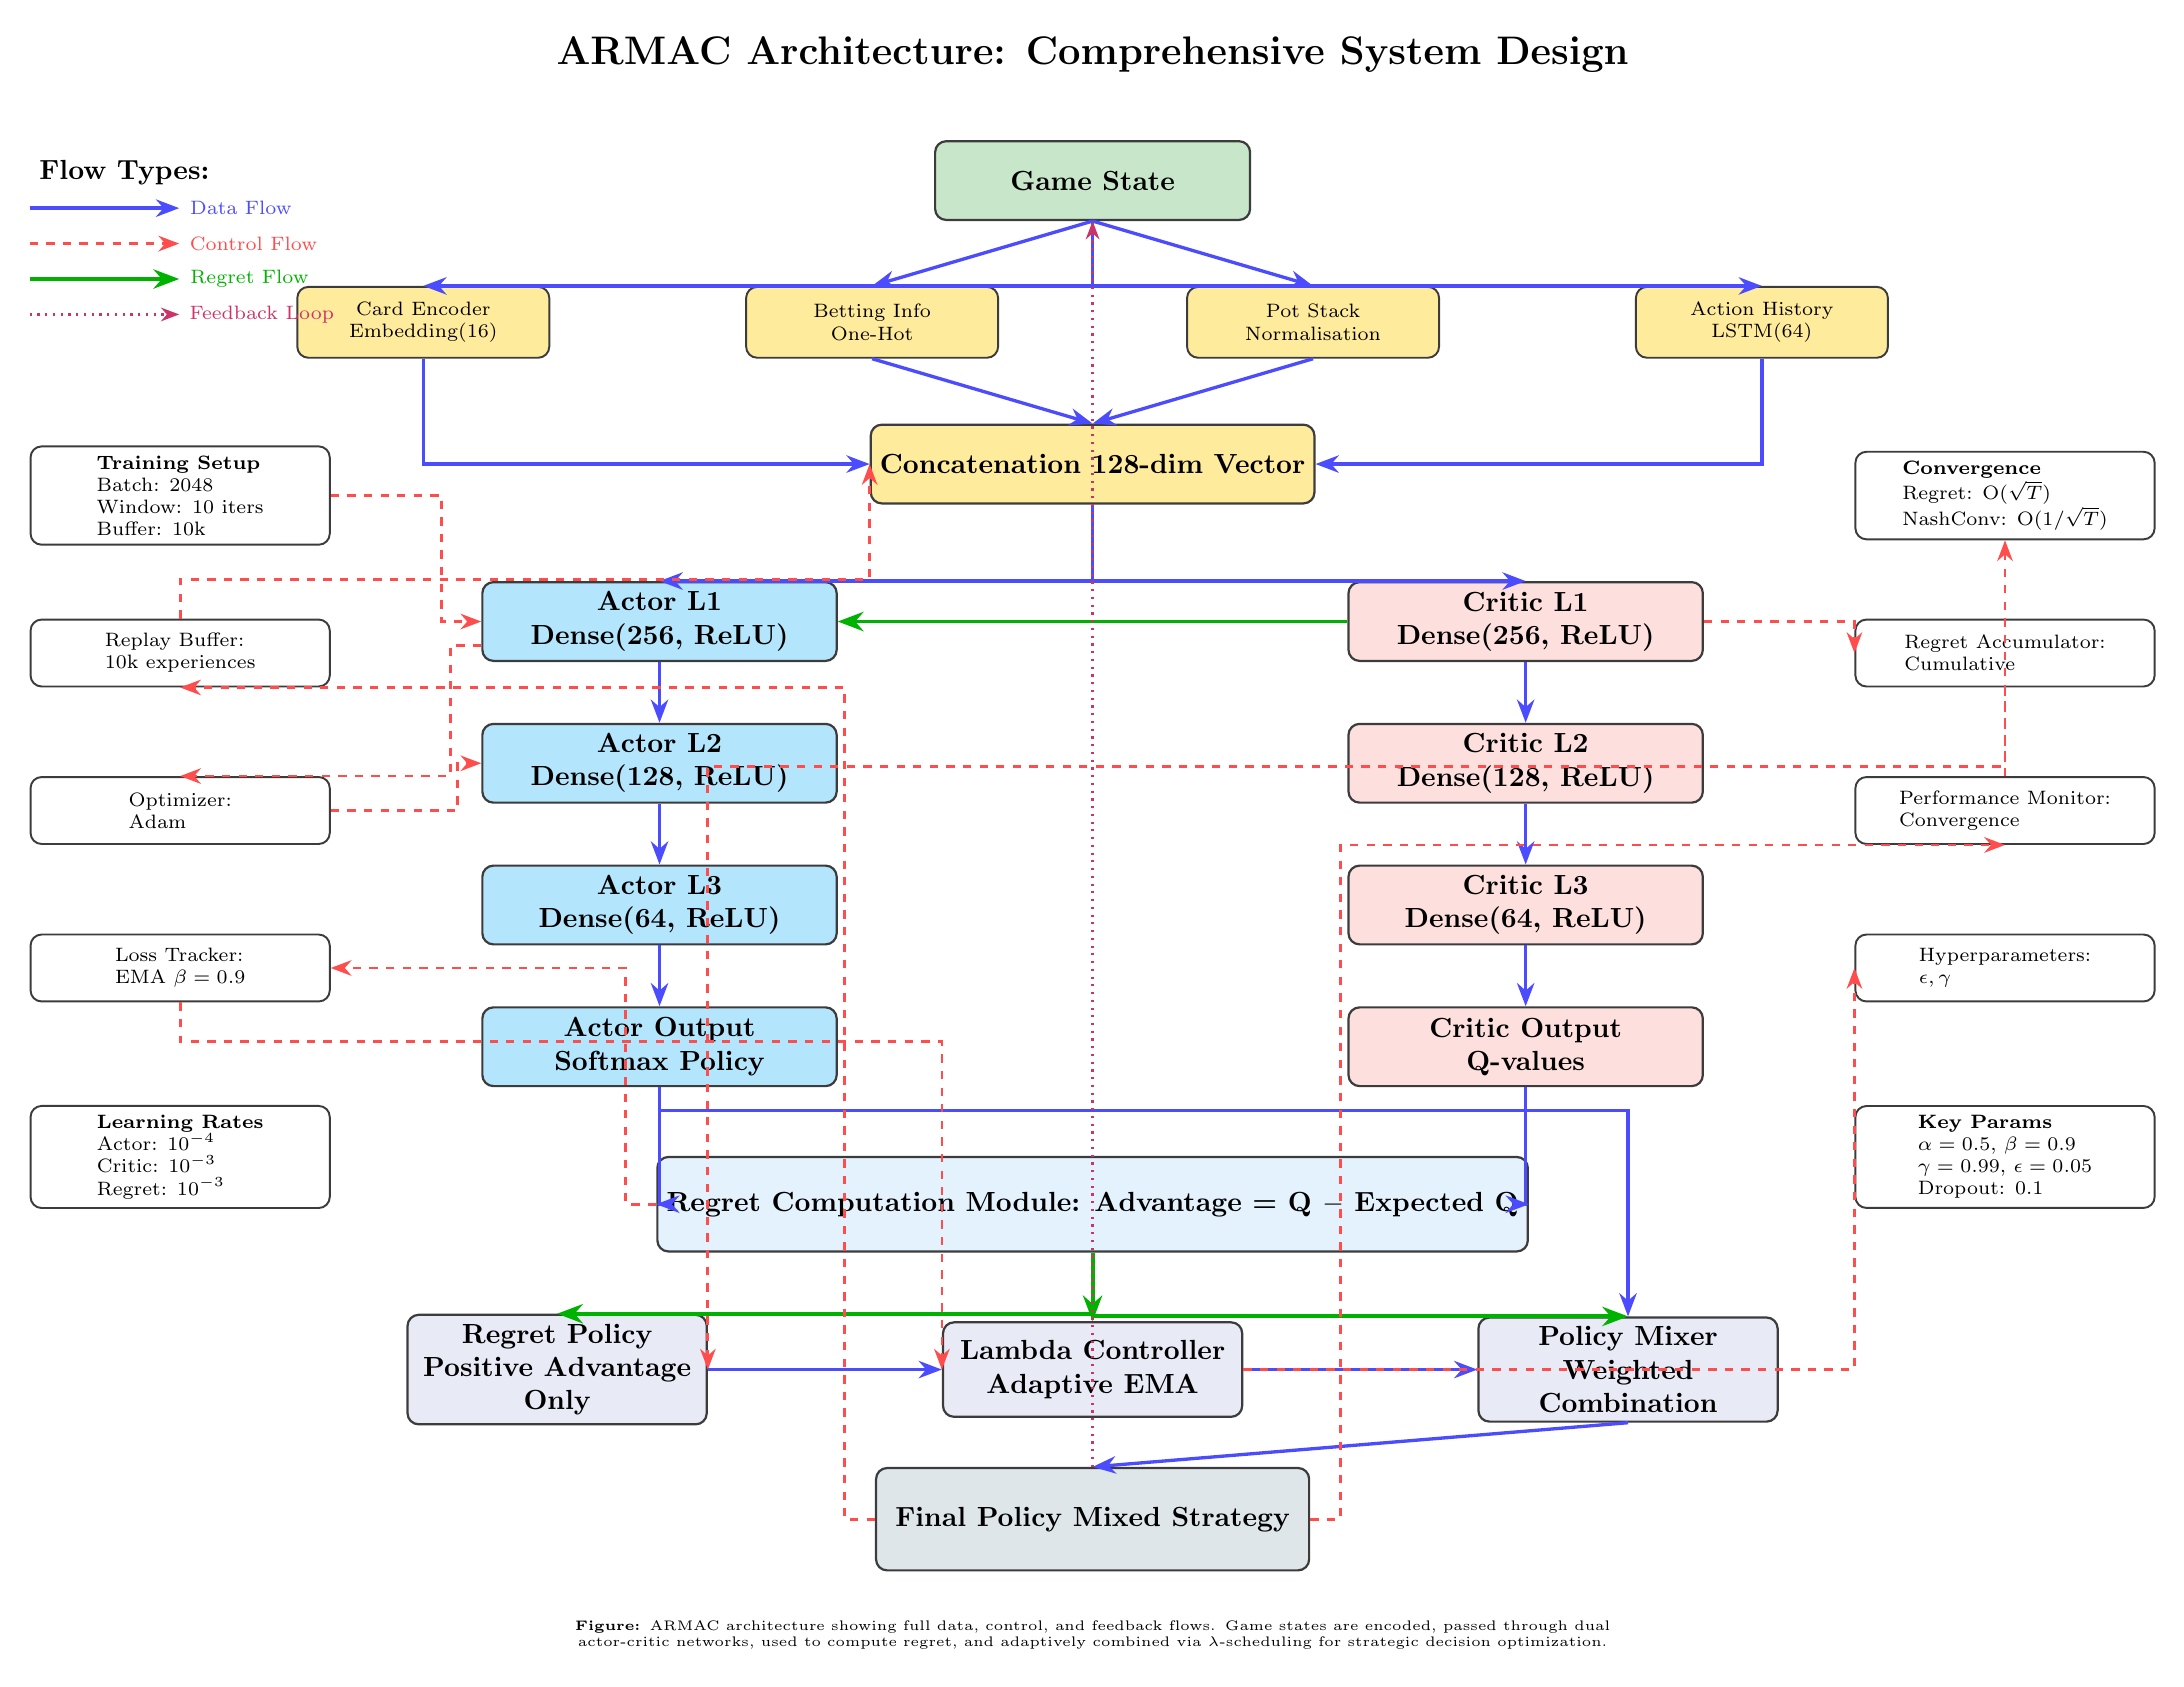
\begin{tikzpicture}[node distance=1.5cm and 0.8cm]
% Define positions with better spacing
\def\actorX{-5.5}
\def\criticX{5.5}
\def\centerlineX{0}
\def\leftMargin{-13.5}
\def\rightMargin{13.5}

% =====================================================
% TITLE
\node[font=\Large\bfseries] at (\centerlineX,10.8) {ARMAC Architecture: Comprehensive System Design};

% INPUT + ENCODERS
\node[input] (gamestate) at (\centerlineX,9.2) {Game State};
\node[encoder] (cardenc) at (-8.5,7.4) {Card Encoder\\Embedding(16)};
\node[encoder] (betenc) at (-2.8,7.4) {Betting Info\\One-Hot};
\node[encoder] (potenc) at (2.8,7.4) {Pot Stack\\Normalisation};
\node[encoder] (histenc) at (8.5,7.4) {Action History\\LSTM(64)};
\node[concat] (concat) at (\centerlineX,5.6) {Concatenation 128-dim Vector};

% ACTOR NETWORK (left side)
\node[actor] (actor_l1) at (\actorX,3.6) {Actor L1\\Dense(256, ReLU)};
\node[actor] (actor_l2) at (\actorX,1.8) {Actor L2\\Dense(128, ReLU)};
\node[actor] (actor_l3) at (\actorX,0.0) {Actor L3\\Dense(64, ReLU)};
\node[actor] (actor_out) at (\actorX,-1.8) {Actor Output\\Softmax Policy};

% CRITIC NETWORK (right side)
\node[critic] (critic_l1) at (\criticX,3.6) {Critic L1\\Dense(256, ReLU)};
\node[critic] (critic_l2) at (\criticX,1.8) {Critic L2\\Dense(128, ReLU)};
\node[critic] (critic_l3) at (\criticX,0.0) {Critic L3\\Dense(64, ReLU)};
\node[critic] (critic_out) at (\criticX,-1.8) {Critic Output\\Q-values};

% REGRET MODULE
\node[regretmod] (regret_module) at (\centerlineX,-3.8) {Regret Computation Module: Advantage = Q $-$ Expected Q};

% POLICY MODULES (bottom row - evenly spaced)
\node[policymod] (regret_policy) at (-6.8,-5.9) {Regret Policy\\Positive Advantage\\Only};
\node[policymod] (lambda_ctrl) at (\centerlineX,-5.9) {Lambda Controller\\Adaptive EMA};
\node[policymod] (policy_mixer) at (6.8,-5.9) {Policy Mixer\\Weighted\\Combination};

\node[output] (final_policy) at (\centerlineX,-7.8) {Final Policy Mixed Strategy};

% LEFT SIDE MODULES - Better vertical spacing
\node[smallmodule, anchor=west] (train_setup) at (\leftMargin,5.2) {\textbf{Training Setup}\\Batch: 2048\\Window: 10 iters\\Buffer: 10k};
\node[smallmodule, anchor=west] (replay) at (\leftMargin,3.2) {Replay Buffer:\\10k experiences};
\node[smallmodule, anchor=west] (opt) at (\leftMargin,1.2) {Optimizer:\\Adam};
\node[smallmodule, anchor=west] (loss) at (\leftMargin,-0.8) {Loss Tracker:\\EMA $\beta=0.9$};
\node[smallmodule, anchor=west] (lrate) at (\leftMargin,-3.2) {\textbf{Learning Rates}\\Actor: $10^{-4}$\\Critic: $10^{-3}$\\Regret: $10^{-3}$};

% RIGHT SIDE MODULES - Aligned with left side
\node[smallmodule, anchor=east] (converge) at (\rightMargin,5.2) {\textbf{Convergence}\\Regret: O($\sqrt{T}$)\\NashConv: O($1/\sqrt{T}$)};
\node[smallmodule, anchor=east] (accum) at (\rightMargin,3.2) {Regret Accumulator:\\Cumulative};
\node[smallmodule, anchor=east] (perf) at (\rightMargin,1.2) {Performance Monitor:\\Convergence};
\node[smallmodule, anchor=east] (hyper) at (\rightMargin,-0.8) {Hyperparameters:\\$\epsilon, \gamma$};
\node[smallmodule, anchor=east] (keyparam) at (\rightMargin,-3.2) {\textbf{Key Params}\\$\alpha=0.5$, $\beta=0.9$\\$\gamma=0.99$, $\epsilon=0.05$\\Dropout: 0.1};

% ================== CONNECTIONS (ALL STRAIGHT LINES) ==================
% Data Flows from Game State to Encoders
\draw[dataflow] (gamestate.south) |- (cardenc.north);
\draw[dataflow] (gamestate.south) -- (betenc.north);
\draw[dataflow] (gamestate.south) -- (potenc.north);
\draw[dataflow] (gamestate.south) |- (histenc.north);

% Encoders to Concatenation
\draw[dataflow] (cardenc.south) |- (concat.west);
\draw[dataflow] (betenc.south) -- (concat.north);
\draw[dataflow] (potenc.south) -- (concat.north);
\draw[dataflow] (histenc.south) |- (concat.east);

% Concat to Networks
\draw[dataflow] (concat.south) |- (actor_l1.north);
\draw[dataflow] (concat.south) |- (critic_l1.north);

% Actor Network Flow
\draw[dataflow] (actor_l1) -- (actor_l2);
\draw[dataflow] (actor_l2) -- (actor_l3);
\draw[dataflow] (actor_l3) -- (actor_out);

% Critic Network Flow
\draw[dataflow] (critic_l1) -- (critic_l2);
\draw[dataflow] (critic_l2) -- (critic_l3);
\draw[dataflow] (critic_l3) -- (critic_out);

% Networks to Regret Module
\draw[dataflow] (actor_out.south) |- (regret_module.west);
\draw[dataflow] (critic_out.south) |- (regret_module.east);

% Regret Module to Policy Modules
\draw[regretflow] (regret_module.south) |- (regret_policy.north);
\draw[regretflow] (regret_module.south) -- (lambda_ctrl.north);
\draw[regretflow] (regret_module.south) |- (policy_mixer.north);

% Actor Output to Policy Mixer (around the side)
\draw[dataflow] (actor_out.south) |- ([yshift=-0.3cm]actor_out.south) -| (policy_mixer.north);

% Policy Module Connections
\draw[dataflow] (regret_policy.east) -- (lambda_ctrl.west);
\draw[dataflow] (lambda_ctrl.east) -- (policy_mixer.west);

% Policy Mixer to Final Policy
\draw[dataflow] (policy_mixer.south) -- (final_policy.north);

% ========== CONTROL FLOWS (ALL STRAIGHT) ==========
% LEFT SIDE
% Training Setup to Actor
\draw[controlflow] (train_setup.east) -| ([xshift=-0.5cm]actor_l1.west) -- (actor_l1.west);

% Final Policy to Replay Buffer
\draw[controlflow] (final_policy.west) -| ([xshift=-11,yshift=0cm]final_policy.west) |- (replay.south);

% Replay Buffer to Concat
\draw[controlflow] (replay.north) |- ([yshift=0.5cm]replay.north) -| (concat.west);

% Optimizer connections
\draw[controlflow] ([yshift=-0.3cm]actor_l1.west) -| ([xshift=-11,yshift=-0.3cm]actor_l1.west) |- (opt.north);
\draw[controlflow] (opt.east) -| ([xshift=-0.3cm]actor_l2.west) -- (actor_l2.west);

% Loss Tracker
\draw[controlflow] (regret_module.west) -| ([xshift=-11]regret_module.west) |- (loss.east);
\draw[controlflow] (loss.south) |- ([yshift=-0.5cm]loss.south) -| (lambda_ctrl.west);

% RIGHT SIDE
% Critic to Regret Accumulator
\draw[controlflow] (critic_l1.east) -| (accum.west);

% Regret Accumulator to Regret Policy
\draw[controlflow] (accum.south) |- ([yshift=-1cm]accum.south) -| (regret_policy.east);

% Performance Monitor
\draw[controlflow] (final_policy.east) -| ([xshift=11]final_policy.east) |- (perf.south);
\draw[controlflow] (perf.north) |- ([yshift=0.5cm]perf.north) -| (converge.south);

% Hyperparameters
\draw[controlflow] (lambda_ctrl.east) -| (hyper.west);

% ========== SPECIAL FLOWS (STRAIGHT) ==========
% Feedback Loop - Critic to Actor (Green)
\draw[regretflow] (critic_l1.west) -- (actor_l1.east);

% Feedback Loop - Final Policy to Game State (Purple dotted)
\draw[feedbackflow] (final_policy.north) -- (gamestate.south);

% ================== LEGEND ==================
\node[anchor=west, font=\bfseries] at (\leftMargin,9.3) {Flow Types:};
\draw[dataflow] (\leftMargin,8.85)--(-11.6,8.85) node[right,font=\scriptsize]{Data Flow};
\draw[controlflow] (\leftMargin,8.4)--(-11.6,8.4) node[right,font=\scriptsize]{Control Flow};
\draw[regretflow] (\leftMargin,7.95)--(-11.6,7.95) node[right,font=\scriptsize]{Regret Flow};
\draw[feedbackflow] (\leftMargin,7.5)--(-11.6,7.5) node[right,font=\scriptsize]{Feedback Loop};

% Caption
\node[below=0.5cm of final_policy,font=\tiny,text width=17cm,align=center] {
\textbf{Figure:} ARMAC architecture showing full data, control, and feedback flows. Game states are encoded, passed through dual actor-critic networks, used to compute regret, and adaptively combined via $\lambda$-scheduling for strategic decision optimization.
};

\end{tikzpicture}
\end{document}
